\documentclass[aspectratio=169,10pt]{beamer}
\usetheme{Madrid}
\usepackage[T1]{fontenc}
\usepackage{amsmath,amssymb}
\usepackage{booktabs}
\usepackage{tikz}
\usepackage{graphicx}
\usetikzlibrary{arrows.meta,positioning}
\setbeamertemplate{navigation symbols}{}
\setbeamertemplate{footline}{}
\setbeamerfont{block title}{size=\small}
\setbeamertemplate{itemize items}[circle]
\setlength{\tabcolsep}{5pt}

\title{Which Truth Does the Slide See?}
\subtitle{Auditing what pathology foundation models learn when IHC, mRNA and protein disagree\\[3pt]\small Project Update: Weeks 1--3}
\author{Aman Uniyal \and Aman Srivastava}
\institute{Topics in AI for Healthcare, IIIT Hyderabad\\[2pt]
  \footnotesize Base project: Kamineni -- Multimodal Breast Cancer Diagnostic \& Outcome Assistant}
\date{\today}

\begin{document}

%===================================================================
\begin{frame}
  \titlepage
\end{frame}

%===================================================================
\begin{frame}[t]{Week 1: Proposal -- Problem, Question \& Pipeline}
\footnotesize
\begin{columns}[T]
\begin{column}{0.48\textwidth}
\begin{block}{Clinical problem}
\begin{itemize}
  \item ER/PR/HER2 status drives therapy and is measured by \textbf{IHC}.
  \item IHC often disagrees with mRNA; on HER2 0 vs 1+ pathologists agree in only $\sim$26\% of cases.
  \item H\&E models learn whatever label they are given: \textbf{which biological truth do they track?}
\end{itemize}
\end{block}
\begin{alertblock}{Research question}
When IHC, RNA and PAM50 disagree, which one does an H\&E foundation model follow, and does it depend on the slide type?
\end{alertblock}
\end{column}
\begin{column}{0.48\textwidth}
\begin{block}{Five experiments}
\begin{itemize}
  \item[\textbf{1a}] Is the IHC or the RNA label more predictable?
  \item[\textbf{1b}] On discordant cases, which side does the model take?
  \item[\textbf{1c}] Does it change from FFPE to frozen slides?
  \item[\textbf{1d}] Is HER2 0 vs 1+ visible in H\&E at all?
  \item[\textbf{1e}] Do two frozen slides of one tumour agree?
\end{itemize}
\end{block}
\end{column}
\end{columns}

\vspace{8pt}
\centering
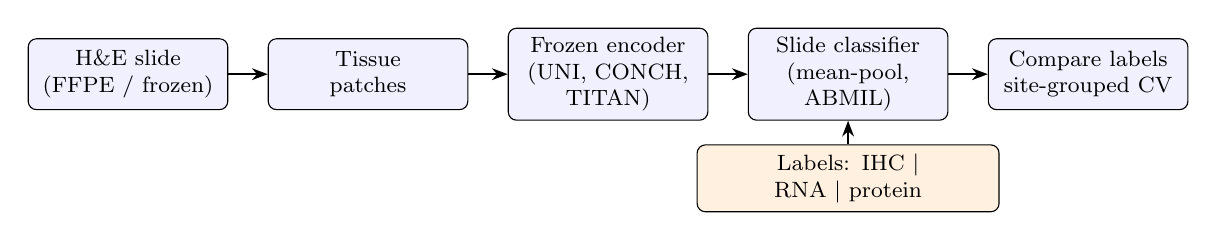
\begin{tikzpicture}[
  box/.style={draw, rounded corners=3pt, fill=blue!6, align=center, font=\footnotesize,
              text width=2.3cm, minimum height=0.9cm},
  lab/.style={draw, rounded corners=3pt, fill=orange!12, align=center, font=\footnotesize,
              text width=3.6cm, minimum height=0.6cm},
  arr/.style={-{Stealth[length=2mm]}, thick}, node distance=0.5cm]
  \node[box] (wsi) {H\&E slide\\(FFPE / frozen)};
  \node[box, right=of wsi] (patch) {Tissue\\patches};
  \node[box, right=of patch] (enc) {Frozen encoder\\(UNI, CONCH, TITAN)};
  \node[box, right=of enc] (head) {Slide classifier\\(mean-pool, ABMIL)};
  \node[box, right=of head] (out) {Compare labels\\site-grouped CV};
  \node[lab, below=0.3cm of head] (labels) {Labels: IHC $\mid$ RNA $\mid$ protein};
  \draw[arr] (wsi) -- (patch);
  \draw[arr] (patch) -- (enc);
  \draw[arr] (enc) -- (head);
  \draw[arr] (head) -- (out);
  \draw[arr] (labels) -- (head);
\end{tikzpicture}
\end{frame}

%===================================================================
\begin{frame}[t]{Week 1: Dataset -- TCGA-BRCA}
\footnotesize
\begin{columns}[T]
\begin{column}{0.44\textwidth}
\begin{block}{Cohort}
\begin{itemize}
  \item 1,097 patients from 40 tissue-source sites (open access).
  \item Labels joined per patient from public metadata: IHC, RNA, PAM50, RPPA protein.
  \item Three slide types per patient:
\end{itemize}
\end{block}
\centering
\begin{tabular}{lr}
\toprule
Slide type & Patients \\
\midrule
FFPE diagnostic (DX) & 1,060 \\
Frozen top (TS) & 1,043 \\
Frozen bottom (BS) & 427 \\
\bottomrule
\end{tabular}
\end{column}
\begin{column}{0.52\textwidth}
\begin{block}{How often the ``truths'' disagree (no images)}
\centering
\scriptsize
\begin{tabular}{llrc}
\toprule
Marker & Compared & Discordant & mRNA alone $\rightarrow$ IHC (AUC) \\
\midrule
ER & IHC vs RNA & 5.5\% & 0.96 \\
PR & IHC vs RNA & 16.7\% & 0.92 \\
HER2 & IHC/FISH vs amplification & 10.8\% & 0.87 \\
\bottomrule
\end{tabular}
\end{block}
\begin{block}{Notes}
\begin{itemize}
  \item TCGA's HER2 field is noisy $\rightarrow$ we use a strict IHC/FISH rule.
  \item ER discordance is mostly ER-low tumours.
  \item \textbf{All five experiments are feasible} on public data (smallest: 1d, 57 vs 261 cases).
\end{itemize}
\end{block}
\end{column}
\end{columns}
\end{frame}

%===================================================================
\begin{frame}[t]{Week 1: Baselines \& First Results}
\footnotesize
\textbf{Setup:} 3 frozen encoders on the DX slides of 1,055 patients $\rightarrow$ logistic regression on the slide
embedding (TITAN) or on the mean of all patches (UNI, CONCH); 5-fold \textbf{site-grouped} CV, repeated over seeds.
\vspace{3pt}

\centering
\scriptsize
\begin{tabular}{llccc}
\toprule
 & Task & TITAN & UNI v1 & CONCH v1 \\
\midrule
\textbf{1a} & ER: IHC $\rightarrow$ RNA label ($n$=801) & 0.87 $\rightarrow$ \textbf{0.92} & 0.87 $\rightarrow$ \textbf{0.91} & 0.84 $\rightarrow$ \textbf{0.87} \\
AUC & PR: IHC $\rightarrow$ RNA label ($n$=986) & 0.80 $\rightarrow$ 0.79 & 0.80 $\rightarrow$ 0.73 & 0.78 $\rightarrow$ 0.75 \\
 & HER2: clinical $\rightarrow$ amplif. ($n$=478) & 0.68 $\rightarrow$ 0.72 & 0.63 $\rightarrow$ 0.68 & 0.62 $\rightarrow$ 0.68 \\
\midrule
\textbf{1b} & ER discordant ($n$=54) & \textbf{RNA} 39:15** & RNA 34:20 & \textbf{RNA} 35:19* \\
side & PR discordant ($n$=169) & \textbf{IHC} 100:69* & \textbf{IHC} 114:55*** & \textbf{IHC} 108:61*** \\
 & HER2 discordant ($n$=60) & 35:25 & \textbf{amplif.} 44:16*** & \textbf{amplif.} 39:21* \\
\midrule
Ctrl & Shuffled ER labels & 0.46 & 0.51 & 0.46 \\
 & HER2 0 vs low (mRNA alone 0.69) & 0.40 & 0.50 & 0.43 \\
\bottomrule
\end{tabular}

\vspace{1pt}
{\tiny 1b: discordant cases where the model sides with the winning label : the other. Binomial * $p<0.05$, ** $p<0.01$, *** $p<0.001$.
TITAN 5 seeds, UNI/CONCH 3 seeds. ABMIL on UNI patches running on Ada (first seed: ER IHC 0.86 vs RNA 0.91).}

\vspace{3pt}
\raggedright
\begin{columns}[T]
\begin{column}{0.49\textwidth}
\begin{block}{Consistent across all three encoders}
\begin{itemize}
  \item \textbf{ER and HER2:} H\&E tracks the \textbf{molecular} label (mRNA / DNA amplification) more than clinical IHC.
  \item \textbf{PR:} the opposite, the model sides with \textbf{IHC}.
\end{itemize}
\end{block}
\end{column}
\begin{column}{0.49\textwidth}
\begin{alertblock}{Site leakage and HER2-low}
Embeddings identify the hospital 82\% of the time, and the hospital ID alone (no image) predicts the label with
AUC 0.53--0.59. HER2 0 vs 1+ looks learnable with random folds (0.63) but is at chance with site-grouped folds.
\end{alertblock}
\end{column}
\end{columns}
\end{frame}

%===================================================================
\begin{frame}[t]{Week 2: ABMIL Agrees; the PR Reversal Was a Cut-off Artefact}
\footnotesize
\begin{columns}[T]
\begin{column}{0.47\textwidth}
\begin{block}{Attention-MIL (ABMIL), UNI and CONCH patches, 3 seeds}
\centering
\scriptsize
\begin{tabular}{lcc}
\toprule
 & UNI v1 & CONCH v1 \\
\midrule
1a ER: IHC $\rightarrow$ RNA & 0.86 $\rightarrow$ \textbf{0.91} & 0.85 $\rightarrow$ \textbf{0.90} \\
1a HER2: clinical $\rightarrow$ amplif. & 0.67 $\rightarrow$ 0.69 & 0.67 $\rightarrow$ 0.73 \\
1b ER discordant ($n$=54) & RNA 34:20 & \textbf{RNA} 36:18* \\
1b HER2 discordant ($n$=60) & \textbf{amplif.} 47:13*** & 34:26 \\
Shuffled ER (control) & 0.49 & 0.46 \\
HER2 0 vs low & 0.55 & 0.52 \\
\bottomrule
\end{tabular}
\end{block}
\begin{itemize}
  \item ABMIL agrees with mean-pooling: the RNA-defined ER label is more predictable; HER2 calls side with amplification.
  \item HER2-low stays at chance with attention as well.
\end{itemize}
\end{column}
\begin{column}{0.50\textwidth}
\begin{block}{PR: $\Delta$AUC (RNA $-$ IHC label) under two RNA cut-offs}
\centering
\scriptsize
\begin{tabular}{lcc}
\toprule
Model & GMM cut-off & Prevalence-matched \\
\midrule
TITAN & $-$0.006 & +0.033 \\
UNI mean & $-$0.047 & $-$0.008 \\
CONCH mean & $-$0.027 & +0.010 \\
UNI ABMIL & $-$0.058 & $-$0.006 \\
CONCH ABMIL & $-$0.029 & +0.011 \\
\midrule
1b PR discordant & IHC wins ($n$=169) & 61--69 : 64--72 ($n$=133) \\
\bottomrule
\end{tabular}
\end{block}
\begin{alertblock}{PR: no reliable preference}
The GMM cut-off calls more tumours PR-negative than IHC does. With a cut-off matching the IHC prevalence the
gap disappears and the discordant cases split evenly (all five models $p > 0.3$).
\end{alertblock}
\end{column}
\end{columns}
\end{frame}

%===================================================================
\begin{frame}[t]{Week 2: ER-low Tumours Are Read as ER-negative}
\scriptsize
\begin{columns}[T]
\begin{column}{0.55\textwidth}
\begin{block}{ER-discordant cases by subgroup (RNA : IHC side)}
\centering
\begin{tabular}{lcccc}
\toprule
Subgroup & $n$ & TITAN & UNI & CONCH \\
\midrule
IHC+ / RNA$-$ & 34 & 24:10 & 21:13 & 22:12 \\
IHC$-$ / RNA+ & 20 & 15:5 & 13:7 & 13:7 \\
\textbf{ER-low} (IHC+, $<$10\%) & 10 & \textbf{8:2} & \textbf{8:2} & \textbf{8:2} \\
ER 10--39\% stained & 9 & 7:2 & 6:3 & 7:2 \\
\bottomrule
\end{tabular}
\end{block}
\begin{block}{ABMIL attention maps (UNI): 54 discordant + 10 reference patients}
\begin{itemize}
  \item Sides with RNA in \textbf{35 / 54} discordant and \textbf{8 / 10} ER-low cases (references: 8 / 10 correct).
  \item P(ER+) tracks ESR1 expression ($r$ = 0.52); attention is focused and similar across groups.
  \item Both ER-low exceptions are HER2-enriched; all 6 Basal ER-low tumours are called ER$-$.
\end{itemize}
\end{block}
\end{column}
\begin{column}{0.42\textwidth}
\centering
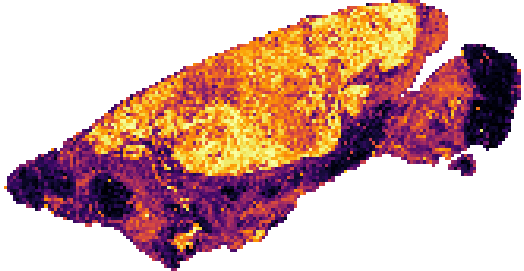
\includegraphics[height=2.3cm]{week1_week2_build/att_TCGA-A2-A4S1.png}\\[1pt]
{\tiny ER-low, RNA$-$, Basal $\rightarrow$ called ER$-$}\\[4pt]
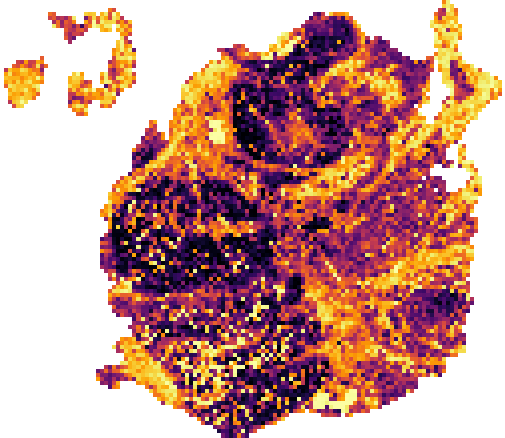
\includegraphics[height=2.0cm]{week1_week2_build/att_TCGA-AR-A0TX.png}\\[1pt]
{\tiny Exception: ER-low, RNA$-$, HER2-enriched $\rightarrow$ called ER+}\\[2pt]
{\tiny Colour = attention percentile (bright = high).}
\end{column}
\end{columns}
\end{frame}

%===================================================================
\begin{frame}[t]{Week 2: Frozen Slides -- Results of 1c and 1e}
\footnotesize
1,515 frozen sections (TS = above, BS = below the sequenced tissue) encoded with the same pipeline as the FFPE (DX)
features (verified: cosine 1.0000 on 46 re-extracted DX slides). UNI mean-pool, same patients, same site-grouped folds.

\vspace{6pt}
\begin{columns}[T]
\begin{column}{0.56\textwidth}
\begin{block}{1c: does the answer change from FFPE to frozen? ($n$ = 947)}
\centering
\scriptsize
\begin{tabular}{lcccc}
\toprule
$\Delta$AUC (molecular $-$ IHC) & DX & TS & TS $-$ DX & $p$ \\
\midrule
\textbf{ER: RNA $-$ IHC} & +0.032 & +0.032 & \textbf{0.000} & 0.98 \\
PR: RNA $-$ IHC (matched) & $-$0.003 & +0.026 & +0.029 & 0.12 \\
HER2: amp. $-$ strict & +0.045 & +0.014 & $-$0.030 & 0.44 \\
\bottomrule
\end{tabular}\\[2pt]
{\tiny TS $-$ DX = interaction; ER 95\% CI $-$0.024 to +0.024.}
\end{block}
\begin{itemize}
  \item The frozen slide next to the sequenced tissue prefers RNA \textbf{exactly as much} as the FFPE slide:
        the ER result is not a tissue-sampling artefact.
  \item ER-discordant patients: frozen slides side with RNA \textbf{39 : 13} ($p$ = 0.0004; FFPE 34 : 18).
\end{itemize}
\end{column}
\begin{column}{0.41\textwidth}
\begin{block}{1e: do two frozen sections of one tumour agree? (373 pairs)}
\centering
\scriptsize
\begin{tabular}{lccc}
\toprule
ER model trained on & ICC & $\kappa$ & Calls flipped \\
\midrule
IHC label & 0.87 & 0.73 & 10.9\% \\
RNA label & 0.89 & 0.81 & 7.6\% \\
\bottomrule
\end{tabular}
\end{block}
\begin{itemize}
  \item Predictions agree well, but \textbf{$\sim$1 in 10 ER calls flips} between sections a few mm apart.
  \item Flipped cases sit at the 0.5 threshold; the RNA-trained model is somewhat more reproducible.
\end{itemize}
\end{column}
\end{columns}
\end{frame}

%===================================================================
\begin{frame}[t]{Week 3: Zero-shot CONCH Prompts Cannot Read Receptor Status}
\footnotesize
\begin{columns}[T]
\begin{column}{0.45\textwidth}
\begin{block}{Label-free audit with CONCH (vision--language)}
\begin{itemize}
  \item Each patch is scored against \textbf{text prompts}, no training labels:
        e.g.\ ``estrogen receptor positive'' vs ``negative breast carcinoma''.
  \item 22 prompt templates $\times$ class names; patient score = top-100 patches.
  \item ER prompt sets: all words, receptor words only, subtype words only (``luminal'' vs ``basal-like'').
  \item Check first: the public CONCH features are taken \textbf{before} the image--text projection
        (cosine 1.0000 on 5 re-extracted slides) $\rightarrow$ projection applied before scoring.
\end{itemize}
\end{block}
\end{column}
\begin{column}{0.52\textwidth}
\begin{block}{Zero-shot AUC against each reference (top-k pooling)}
\centering
\scriptsize
\begin{tabular}{llcc}
\toprule
Marker & Prompt set & vs IHC & vs molecular \\
\midrule
ER ($n$=989) & all words & 0.51 & 0.51 (RNA) \\
 & receptor words & 0.48 & 0.46 (RNA) \\
 & subtype words & 0.52 & 0.53 (RNA) \\
PR ($n$=986) & receptor words & 0.50 & 0.51 (RNA) \\
HER2 ($n$=568) & receptor words & 0.53 & 0.54 (amplif.) \\
\bottomrule
\end{tabular}\\[2pt]
{\tiny Mean pooling: ER AUC 0.40--0.46. 1b counts swing with prompt set and pooling (ER 19:35 to 34:20).}
\end{block}
\begin{alertblock}{No label-free auditor}
Every prompt set is at chance against \textbf{every} reference: CONCH's text side does not know what
``ER-positive'' looks like. Named molecular markers are not grounded in the model, a useful negative result for
vision--language models in pathology.
\end{alertblock}
\end{column}
\end{columns}
\end{frame}

%===================================================================
\begin{frame}[t]{Week 3: 14 Named Concepts Reproduce the RNA Preference}
\footnotesize
Zero-shot CONCH share of 14 concepts per slide (tubules, low-grade nuclei, pleomorphism, mitoses, necrosis,
lymphocytes, apocrine, solid sheets, lobular, mucin, stroma, adipose, DCIS, normal breast) $\rightarrow$ logistic
regression, same site-grouped folds, 5 seeds.

\vspace{6pt}
\begin{columns}[T]
\begin{column}{0.56\textwidth}
\begin{block}{Concept-only model: AUC with IHC $\rightarrow$ molecular label}
\centering
\scriptsize
\begin{tabular}{lccc}
\toprule
Comparison & $n$ & AUC & $\Delta$AUC (95\% CI) \\
\midrule
\textbf{ER: RNA $-$ IHC} & 989 & 0.82 $\rightarrow$ \textbf{0.86} & \textbf{+0.036} (+0.010, +0.065) \\
ER: RPPA $-$ IHC & 802 & 0.81 $\rightarrow$ \textbf{0.86} & \textbf{+0.046} (+0.018, +0.076) \\
PR: RNA $-$ IHC (matched) & 986 & 0.74 $\rightarrow$ 0.76 & +0.026 ($-$0.008, +0.060) \\
HER2: amp. $-$ strict & 568 & 0.62 $\rightarrow$ 0.66 & +0.034 ($-$0.020, +0.091) \\
\midrule
1b ER discordant & 54 & \multicolumn{2}{c}{\textbf{RNA 36 : 18*}} \\
1b HER2 discordant & 60 & \multicolumn{2}{c}{amplif.\ 38 : 22 ($p$ = 0.052)} \\
\bottomrule
\end{tabular}
\end{block}
\begin{itemize}
  \item Same ER gain as the 1,024-dim UNI model (+0.036), with AUCs only $\sim$0.06 lower.
\end{itemize}
\end{column}
\begin{column}{0.41\textwidth}
\begin{block}{ER model weights (standardised)}
\centering
\scriptsize
\begin{tabular}{lcc}
\toprule
Concept & IHC label & RNA label \\
\midrule
Tubules & +0.45 & \textbf{+0.86} \\
Lobular pattern & +0.59 & +0.70 \\
Pleomorphism & $-$0.68 & \textbf{$-$0.94} \\
Necrosis & $-$0.83 & \textbf{$-$1.12} \\
Lymphocytes & $-$0.49 & $-$0.47 \\
\bottomrule
\end{tabular}
\end{block}
\begin{alertblock}{Inference}
The RNA preference lives in \textbf{ordinary, nameable morphology} (grade and differentiation); the RNA label is more
tightly tied to it than the IHC label.
\end{alertblock}
\end{column}
\end{columns}
\end{frame}

%===================================================================
\begin{frame}[t]{Week 3: Concepts Describe Who the Discordant Patients Are}
\footnotesize
\begin{block}{Mean concept share per group (z-score; 0 = cohort average)}
\centering
\scriptsize
\begin{tabular}{lccccccc}
\toprule
Group & $n$ & Pleomorphism & Necrosis & Lymphocytes & Apocrine & Tubules & Normal breast \\
\midrule
Concordant ER+ & 729 & $-$0.27 & $-$0.21 & $-$0.17 & $-$0.05 & +0.06 & +0.06 \\
Concordant ER$-$ & 206 & +0.88 & +0.74 & +0.55 & $-$0.01 & $-$0.22 & $-$0.26 \\
IHC+ / RNA$-$, Basal & 15 & \textbf{+2.09} & \textbf{+1.10} & +0.78 & $-$0.10 & $-$0.36 & $-$0.52 \\
IHC+ / RNA$-$, HER2-enriched & 11 & $-$0.25 & $-$0.23 & $-$0.25 & \textbf{+0.79} & $-$0.32 & $-$0.44 \\
IHC$-$ / RNA+ & 20 & $-$0.27 & $-$0.13 & $-$0.02 & $-$0.21 & +0.06 & +0.53 \\
\bottomrule
\end{tabular}
\end{block}

\begin{columns}[T]
\begin{column}{0.48\textwidth}
\begin{itemize}
  \item \textbf{Basal IHC+/RNA$-$} tumours look \emph{more} ER-negative than the typical ER-negative tumour
        (extreme pleomorphism and necrosis) $\rightarrow$ all 15 called ER$-$.
  \item \textbf{IHC$-$/RNA+} tumours look like concordant ER+ tumours (low grade, more normal breast)
        $\rightarrow$ called ER+.
\end{itemize}
\end{column}
\begin{column}{0.48\textwidth}
\begin{alertblock}{The HER2-enriched exception}
IHC+/RNA$-$ HER2-enriched tumours have the \textbf{highest apocrine share} of any group and none of the high-grade
features: this matches 8 / 11 called ER+ and the apocrine-like cells under ABMIL attention (Week 2).
Lead only ($n$ = 11).
\end{alertblock}
\end{column}
\end{columns}
\end{frame}

%===================================================================
\begin{frame}[t]{Week 3: ABMIL 1c -- FFPE vs Frozen ``No Change'' Holds}
\footnotesize
ABMIL (UNI patches, $\le$4,096 per slide) trained separately on FFPE (DX) and frozen (TS) bags of the same 947 patients;
same site-grouped folds, 3 seeds. Mean-pool rows from Week 2 for comparison.

\vspace{6pt}
\begin{columns}[T]
\begin{column}{0.60\textwidth}
\begin{block}{1c: $\Delta$AUC (molecular $-$ IHC) on DX and TS, and the interaction}
\centering
\scriptsize
\begin{tabular}{llcccc}
\toprule
Comparison & Head & DX & TS & TS $-$ DX (95\% CI) & $p$ \\
\midrule
\textbf{ER: RNA $-$ IHC} & mean & +0.032 & +0.032 & 0.000 ($-$0.024, +0.024) & 0.98 \\
 & \textbf{ABMIL} & +0.011 & +0.029 & \textbf{+0.018} ($-$0.008, +0.046) & 0.18 \\
ER: RPPA $-$ IHC & mean & +0.041 & +0.007 & $-$0.035 ($-$0.066, $-$0.001) & 0.045 \\
 & ABMIL & +0.010 & +0.023 & +0.013 ($-$0.020, +0.047) & 0.45 \\
PR: RNA $-$ IHC (matched) & mean & $-$0.003 & +0.026 & +0.029 ($-$0.007, +0.066) & 0.12 \\
 & ABMIL & $-$0.017 & +0.025 & +0.042 (+0.005, +0.079) & 0.031 \\
HER2: amp. $-$ strict & mean & +0.045 & +0.014 & $-$0.030 ($-$0.110, +0.046) & 0.44 \\
 & ABMIL & $-$0.003 & +0.031 & +0.034 ($-$0.047, +0.116) & 0.39 \\
\bottomrule
\end{tabular}\\[2pt]
{\tiny ABMIL ER AUC: DX 0.91 $\rightarrow$ 0.92, TS 0.90 $\rightarrow$ 0.93 (IHC $\rightarrow$ RNA label).}
\end{block}
\end{column}
\begin{column}{0.37\textwidth}
\begin{itemize}
  \item \textbf{ER:} no FFPE vs frozen change with ABMIL either; the CI is wider but stays inside $\pm$0.05 AUC.
  \item ABMIL narrows the IHC--RNA gap on FFPE (+0.011) but not on the frozen slide (+0.029).
  \item The mean-pool ER-RPPA interaction ($p$ = 0.045) \textbf{does not replicate} $\rightarrow$ not robust.
  \item PR leans the same way with both heads: a lead, not a claim.
\end{itemize}
\begin{alertblock}{Inference}
The ER result is not a tissue-sampling or pooling artefact: it holds for both slide types and both heads.
\end{alertblock}
\end{column}
\end{columns}
\end{frame}

%===================================================================
\begin{frame}[t]{Week 3: ABMIL 1b -- Frozen Slides Side More with RNA}
\footnotesize
1b on the patients who have both slide types: train on concordant patients, score the discordant ones
(molecular : IHC side; binomial vs 50 : 50).

\vspace{6pt}
\begin{columns}[T]
\begin{column}{0.58\textwidth}
\begin{block}{1b: DX vs TS, mean-pool vs ABMIL}
\centering
\scriptsize
\begin{tabular}{lccccc}
\toprule
 & & \multicolumn{2}{c}{UNI mean-pool} & \multicolumn{2}{c}{UNI ABMIL} \\
Discordant pair & $n$ & DX & TS & DX & TS \\
\midrule
\textbf{ER: IHC vs RNA} & 52 & 34:18* & \textbf{39:13***} & 34:18* & \textbf{41:11***} \\
HER2: strict vs amplif. & 56 & 38:18* & 36:20* & 40:16** & 45:11*** \\
PR: IHC vs RNA (matched) & 127 & 60:67 & 73:54 & 60:67 & 69:58 \\
\bottomrule
\end{tabular}\\[2pt]
{\tiny * $p<0.05$, ** $p<0.01$, *** $p<0.001$.}
\end{block}
\begin{itemize}
  \item Both heads give the \textbf{same FFPE count} (34 : 18) and a \textbf{stronger RNA side on the frozen slide}
        (39 and 41 of 52).
  \item ABMIL, DX $\rightarrow$ TS: only 1 patient moves towards IHC, 8 towards RNA.
\end{itemize}
\end{column}
\begin{column}{0.39\textwidth}
\begin{alertblock}{Inference}
The frozen section is cut next to the tissue that was RNA-sequenced, so it sees the same tumour state the RNA label
measured: the model's RNA side gets stronger there.
\end{alertblock}
\begin{block}{Other markers}
\begin{itemize}
  \item HER2 follows amplification on both slide types with both heads.
  \item PR: no preference with either head.
\end{itemize}
\end{block}
\end{column}
\end{columns}
\end{frame}

%===================================================================
\begin{frame}[t]{Week 3: ABMIL 1e -- About 1 in 10 Calls Still Flip}
\footnotesize
1e: ER model trained on the top section (TS) of out-of-fold patients, applied to both sections (TS and BS) of each
tumour; bootstrap 95\% CIs.

\vspace{6pt}
\begin{columns}[T]
\begin{column}{0.62\textwidth}
\begin{block}{Agreement between the two sections of one tumour}
\centering
\scriptsize
\begin{tabular}{llcccc}
\toprule
ER model & Head & ICC (95\% CI) & $\kappa$ & Calls flipped (95\% CI) & AUC TS / BS \\
\midrule
IHC label & mean & 0.87 (0.84, 0.90) & 0.73 & 10.9\% (7.9, 14.1) & 0.89 / 0.88 \\
 & ABMIL & 0.81 (0.77, 0.85) & 0.78 & 7.9\% (5.2, 10.6) & 0.89 / 0.89 \\
RNA label & mean & 0.89 (0.87, 0.91) & 0.81 & 7.6\% (4.9, 10.4) & 0.94 / 0.94 \\
 & ABMIL & 0.86 (0.82, 0.88) & 0.77 & 8.7\% (6.0, 11.4) & 0.95 / 0.95 \\
\bottomrule
\end{tabular}\\[2pt]
{\tiny 368 / 367 pairs with an out-of-fold prediction.}
\end{block}
\begin{itemize}
  \item ABMIL pushes probabilities towards 0 and 1: lower ICC on the probability scale, but binary calls agree
        as often.
  \item Both sections give the same accuracy: the flips have no direction.
\end{itemize}
\end{column}
\begin{column}{0.35\textwidth}
\begin{alertblock}{Inference}
\textbf{8--11\% of ER calls flip} between two sections of one tumour with either head: section-to-section
variability is a property of the tissue, not of the pooling.
\end{alertblock}
\begin{block}{Correction to Week 2}
``The RNA-trained model is more reproducible'' does \textbf{not} replicate with ABMIL (8.7\% vs 7.9\%):
head-dependent, so we drop it.
\end{block}
\end{column}
\end{columns}
\end{frame}

%===================================================================
\begin{frame}[t]{Plan for the Next Week (Week 4)}
\footnotesize
\begin{columns}[T]
\begin{column}{0.25\textwidth}
\begin{block}{Done in Week 3}
\begin{itemize}
  \item[\checkmark] Zero-shot CONCH prompts (1a, 1b)
  \item[\checkmark] CONCH feature-space check
  \item[\checkmark] 14-concept model
  \item[\checkmark] Concept profiles of discordant groups
  \item[\checkmark] ABMIL on frozen slides: \textbf{1c}, \textbf{1b}, \textbf{1e}
\end{itemize}
\end{block}
\end{column}
\begin{column}{0.32\textwidth}
\begin{block}{Statistics beyond $p$-values}
\begin{itemize}
  \item Effect sizes with CIs (Cohen's $h$, Wilson CIs) and Bayesian $\Delta$AUC
  \item Equivalence test (TOST) for the 1c ``no change'' claim
  \item Bayes factors for the 1b ``which side'' counts
  \item McNemar for paired calls (DX vs TS, TS vs BS)
  \item Agreement beyond $\kappa$ (Gwet's AC1, Bland--Altman)
  \item Calibration against each reference
\end{itemize}
\end{block}
\end{column}
\begin{column}{0.40\textwidth}
\begin{alertblock}{New experiments (foundation-model features, CPU)}
\begin{enumerate}
  \item[\textbf{C}] \textbf{No gold standard:} treat IHC, RNA, protein and the H\&E model as four imperfect raters
        (latent class model); estimate each one's sensitivity / specificity and re-score the models against the
        latent truth.
  \item[\textbf{D}] \textbf{Model as label auditor:} rank patients by model--IHC disagreement; does it find the
        IHC$\neq$RNA tumours (with RNA as an independent check)? Remove the flagged cases and retrain.
  \item[\textbf{G}] \textbf{FFPE $\leftrightarrow$ frozen transfer:} train on one slide type, test on the other;
        AUC drop, calibration shift, does the RNA preference survive?
\end{enumerate}
\end{alertblock}
\end{column}
\end{columns}
\end{frame}

\end{document}
